
%%
\section{Kieker Data Bridge}

% FRAME
\begin{frame}[fragile]
\frametitle{Kieker Data Bridge}
\begin{figure}
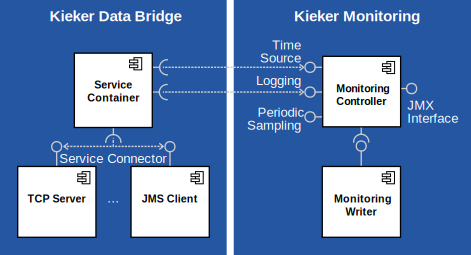
\includegraphics[width=\textwidth]{images/kieker-data-bridge}
\end{figure}
\end{frame}

% FRAME
\begin{frame}[fragile]
\frametitle{Service Connectors}
\structure{TCP Client}  Connects to a remote service on startup
\vskip1em
\structure{TCP Single Server}  Listens for one client
\vskip1em
\structure{TCP Multi Server}  Handles multiple clients
\vskip1em
\structure{JMS Client}  Connects to a JMS queue
\vskip1em
\structure{JMS Embedded}  Start a JMS service and connects to it
\end{frame}

% FRAME
\begin{frame}[fragile]
\frametitle{Service Container}
\structure{Input}
\begin{itemize}
\item Kieker Configuration
\item Service Connector
\end{itemize}
\vskip1em
\structure{Main Loop}
\begin{enumerate}
\item Setup Kieker
\item Setup service connector
\item Get record
\item goto 3 if not terminated
\item Close service connector
\item Shutdown Kieker
\end{enumerate}
\end{frame}

% FRAME
\begin{frame}[fragile]
\frametitle{Service Container}
\structure{Other Features}
\begin{itemize}
\item Connector respawn
\item Progress monitor support
\item Load record types at startup
\item Embeddable container
\end{itemize}
\end{frame}

% FRAME
\begin{frame}[fragile]
\frametitle{Service Implementations}
\structure{CLI Server}
\begin{itemize}
\item Command line application
\item Read class id mapping from ASCII file
\item Can run as deamon
\end{itemize}
\vskip1em
\structure{Eclipse Plugin}
\begin{itemize}
\item Eclipse job \& run configuration
\item Class mapping setup in run configuration
\end{itemize}
\end{frame}

% FRAME
\begin{frame}[fragile]
\frametitle{Serialization Format}
\structure{General Structure}
\begin{itemize}
\item First value \textbf{type id} (int32)
\item Other values in order of declaration
\begin{description}
\item[Kieker ] fields expressed in TYPES
\item[Other ] reflection API (non static fields)
\end{description}
\end{itemize}
\vskip1em
\structure{References}
\begin{itemize}
\item Id only
\begin{itemize}
\item First byte = 0
\item Second value \textbf{type id} (int32)
\item Unique object run-time id
\end{itemize}
\item Containment
\begin{itemize}
\item First byte = 1
\item Second value \textbf{type id} (int32)
\item Other values in order of declaration (Java only)
\end{itemize}
\end{itemize}
\end{frame}

% FRAME
\begin{frame}[fragile]
\frametitle{Serialization Format}
\structure{Binary Format}
\begin{itemize}
\item Based on \textbf{Java base-types}
\item Byte order \textbf{big endien} (network byte order)
\item String composed of
\begin{description}
\item[length ] 32bit signed integer (int)
\item[data ] variable length byte vector
\end{description}
\end{itemize}
\vskip1em
\structure{Text Format}
\begin{itemize}
\item Semicolon separated value list
\end{itemize}
\end{frame}

% FRAME
\begin{frame}[fragile]
\frametitle{Service Connector API}
\begin{lstlisting}[linebackgroundcolor={\btLstHL<2>{3,4}\btLstHL<3>{6,7}\btLstHL<4>{9,10}},escapechar=@,language=Java]
public interface IServiceConnector {

	/** setup connector */
	void setup() throws Exception;

	/** close connector */
	void close() throws Exception;

	/** get next record */
	IMonitoringRecord deserialize() throws Exception;
}
\end{lstlisting}
\end{frame}

